\documentclass[12pt]{article}

\usepackage[a4paper, margin=1in]{geometry}
\usepackage{graphicx}
\usepackage[absolute, overlay]{textpos}
\usepackage{fancyhdr}
\usepackage{siunitx}
\usepackage{tikz}
\usepackage{pgfplots}
\usetikzlibrary{decorations.pathmorphing}
\usetikzlibrary{math}
\usetikzlibrary{calc}

\pgfplotsset{compat=1.18}

\pagestyle{fancy} %for footers

\newcommand{\customsubject}{}   
\newcommand{\customtitle}{}

\newcounter{questionpartcounter}                  %Setup for question part counter for a,b,c listing
\renewcommand{\thequestionpartcounter}
{\alph{questionpartcounter}}

\newcounter{questionpartpartcounter}                  %Setup for question part  partcounter for a,b,c listing
\renewcommand{\thequestionpartpartcounter}
{\roman{questionpartcounter}}

\pagestyle{fancy} %for footers
\renewcommand{\headrulewidth}{0pt}
\fancyhf{}
\fancyfoot[R]{\thepage}

\newenvironment{worksheet}[2]
{
    
    \global\renewcommand{\customtitle}{#1}
    \global\renewcommand{\customsubject}{#2}


    \begin{textblock*}{5cm}(0.4cm,0.4cm)
   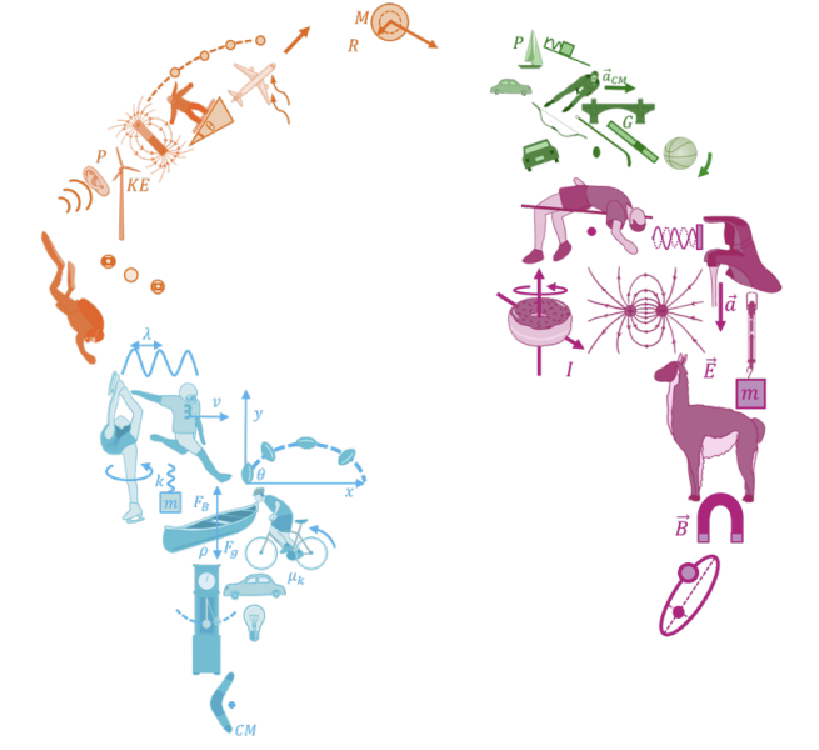
\includegraphics[width=4cm]{include/figures/bmdwlogo}
\end{textblock*}

    \vspace*{-1cm}
    
    {\large\textbf{\begin{center}\customtitle\end{center}}}

    \begin{center}\customsubject\end{center}
    
    \vspace{0.3cm}
    
    \hspace*{-1.5cm}\textbf{Name:\ \rule{4cm}{0.4pt}}\; 
    \textbf{Student \#: \ \rule{3cm}{0.4pt}}\;
    \textbf{Student Email \#: \ \rule{1.53cm}{0.4pt}}

    \vspace{0.5cm}

    
    \begin{enumerate}
}
{
    \end{enumerate}
   % \begin{textblock*}{10cm}(1cm, 28cm) {\footnotesize \scriptsize \customsubject}
    
%\end{textblock*}
}



\newcommand{\question}[2][1cm]{%
    \item
    \setcounter{questionpartcounter}{0}
    \setcounter{questionpartpartcounter}{0}
    {#2}
    \vspace{#1}
}

\newcommand{\questionpart}[2][1cm]{%
    \setcounter{questionpartpartcounter}{0}
    \stepcounter{questionpartcounter}
    (\thequestionpartcounter)~#2
    \vspace{#1}
}

\newcommand{\questionpartpart}[2][1cm]{%
      \stepcounter{questionpartpartcounter}
      \thequestionpartpartcounter.~#2
      \vspace{#1}
}

\newcommand{\operation}[1]{%
{\large $
#1
$}
}



\begin{document}

\begin{worksheet}{Physics Worksheet}{Applying Newton's Laws}


\question[0cm]{Indicate below which of these forces are "real" forces and which are not. Explain the origin of each force and how that determines if the force is fictitious of not:}

\questionpart[0cm]{Gravitational force on a person towards the centre of The Earth}

\textbf{real}
\vspace{1.5cm}

\questionpart[0cm]{Centrifugal force on a mass swinging in a circle}

\textbf{fake}
\vspace{1.5cm}

\questionpart[0cm]{Inertial force on a mass attached to the cieling of an accelerating car via string}

\textbf{fake}
\vspace{1.5cm}

\questionpart[0cm]{Friction force on a beach-ball rolling on sand}

\textbf{real}
\vspace{1.5cm}


\question[0.5cm]{Consider a block traveling along a counter clockwise along a circle that is slowing down. Draw the direction of the linear velocity $\vec{v}$, linear acceleration $\vec{a}$, angular velocity $\vec{\omega}$, and angular acceleratio $\vec{\alpha}$ for the block}

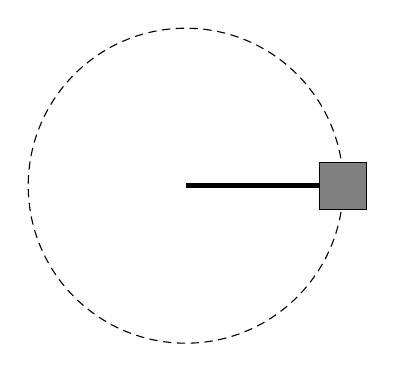
\begin{tikzpicture}

\draw[dash pattern=on 3pt off 2pt] (0,0) circle (2cm);
\draw[fill=gray] (1.7,-0.3) rectangle (2.3, 0.3);
\draw[line width = 2pt, color=black] (0,0)--(1.7,0);
\end{tikzpicture}

\textbf{$\vec{v}$ points up,  $\vec{a}$ points into the circle, $\vec{\omega}$ points out of the page, $\vec{\alpha}$ points into the page.}

\newpage

\question[0.5cm]{A present is placed at rest on a plane that is inclined, at a distance $L$ from the bottom of the incline that makes an angle $\theta$ with the ground. At the bottom of the incline, the box is determined to have a speed $v$. If the box is instead released from a distance of $4L$ from the bottom of the incline, what will its speed at the bottom of the incline be?}


\textbf{$\vec{v_2} = 2\vec{v_1}$}


\vspace{5cm}




\question[0cm]{Imagine you are swinging a bucket full of water attached to a rope in a vertical circle}

\questionpart[0cm]{Where along the trajectory is the tension on the rope the highest?}

\textbf{At the bottom becuase the tension directly opposes the weight of the bucket}
\vspace{4cm}

\questionpart[0cm]{Why doesn't the water spill out of the bucket at the top of the circle? Give two explanations:}

\textbf{1. The normal force, centripidal force and gravitational forces cancel each other out. 2. The water is actually in free-fall, however so is the bucket. and since they are in movement together the water stays within the bucket}
\vspace{2cm}

\questionpart[0cm]{What is the minimum speed required for the water to not spill out of the bucket?}


\textbf{$v=\sqrt{gR}$ where R is the radius of the circular path the bucket is rotating around.}




\end{worksheet}

\end{document}